%!TEX program = xelatex
\documentclass[dvipsnames, svgnames,a4paper,11pt]{book}

% ---------------------------------------------------------------------------------
% --------------------------------------设定--------------------------------------
%---------------------------------------------------------------------------------

% 杨舒云自用LaTex笔记设定集
%下面是一些碎碎念……


% ---------------------------------------------------------------------
% 自定义颜色（流萤主题配色——老婆的颜色！）
\usepackage{xcolor}
\definecolor{fblack}{HTML}{3E324A} % #3e324a（紫黑）
\definecolor{fgrayblue}{HTML}{475D7B} % #475d7b（灰蓝）
\definecolor{fgraygreen}{HTML}{97C6C0} % #97c6c0（灰绿）
\definecolor{fred}{HTML}{E26E1B} % #e26e1b（深橘红）
\definecolor{fsilver}{HTML}{E6E4E0} % #e6e4e0（银白）
\definecolor{fbluegreen}{HTML}{4DF8E8} % #4df8e8（蓝绿）


% ---------------------------------------------------------------------
% 链接
\usepackage{ctex}
\usepackage[top=28mm,bottom=28mm,left=15mm,right=15mm]{geometry}
\usepackage{hyperref} 
\hypersetup{
	colorlinks,
	linktoc = section, % 超链接位置，选项有section, page, all
	linkcolor = fgrayblue, % linkcolor 目录颜色
	citecolor = fgrayblue  % citecolor 引用颜色
}


% ---------------------------------------------------------------------
% 引入必要的包
%A
\usepackage{amsmath,enumerate,multirow,float} % 数学公式，
\usepackage{tabularx}
\usepackage{tabu}
\usepackage{subfig}
\usepackage{fancyhdr}
\usepackage{graphicx} % 插图
\usepackage{wrapfig}  
\usepackage{physics}
\usepackage{appendix}
\usepackage{amsfonts}
%B
\usepackage{mathrsfs} % 字体
\usepackage{calligra}
\usepackage{lipsum}
\usepackage{adjustbox}% 调整表格大小
\usepackage{tabularray} % 绘制表格时可以更加方便添加框线
%C
\usepackage{caption}
\usepackage{authblk}
\usepackage{braket}
\usepackage{amssymb} % 包含更多数学符号
\usepackage[en-US]{datetime2} % 设置日期为美式英语格式
\usepackage{geometry}  % 页面调整


% ---------------------------------------------------------------------
% 对目录、章节标题的设置
\usepackage{titlesec}
\usepackage{titletoc}
% 目录
\renewcommand{\contentsname}{\centerline{\Huge Outline}}

% 定义章节标题格式
\titleformat{\chapter}[block]
{\centering\bfseries\color{fblack}\Huge} % 格式：居中、加粗、Large字体
{PART \thechapter}          % 标题前缀
{1em}                       % 前缀与标题之间的间距
{ }                         % 标题格式
% 设置章节编号格式为罗马数字
\renewcommand{\thechapter}{\Roman{chapter}}

% 自定义章节编号
\renewcommand\thesection{\S\arabic{section}}
\renewcommand\thesubsection{\thesection.\arabic{subsection}}
\renewcommand\thesubsubsection{\S\arabic{section}.\arabic{subsection}.\arabic{subsubsection}}


% 自定义section格式
\titleformat{\section}
{\normalfont\bfseries\color{fgrayblue}\Large} % 设置字体、大小、加粗、颜色
{\thesection} % 设置section编号的格式
{1em} % 编号和标题之间的间距
{}

% 自定义subsection格式
\titleformat{\subsection}
{\normalfont\bfseries\color{fgrayblue}\large} % 设置字体、大小、颜色
{\thesubsection} % 设置subsection编号的格式
{1em} % 编号和标题之间的间距
{}

% 自定义subsubsection格式
\setcounter{secnumdepth}{3}
\titleformat{\subsubsection}
{\normalfont\bfseries\color{fgrayblue}\normalsize} % 设置字体、大小、颜色
{\thesubsubsection} % 设置subsubsection编号的格式
{1em} % 编号和标题之间的间距
{}

% 章节计数器独立于Chapter
\makeatletter
\@addtoreset{section}{chapter}
\@addtoreset{subsection}{chapter}
\@addtoreset{subsubsection}{chapter}
\makeatother


% ---------------------------------------------------------------------
% 颜色盒子
\usepackage{tcolorbox}
\tcbuselibrary{skins, breakable}
% 设置 Key Point 环境
\newtcolorbox{keypoint}[1][]{enhanced, breakable,
	colback=fbluegreen!30!white,colframe=fbluegreen!80!black,colbacktitle = fbluegreen!80!black,
	attach boxed title to top left = {yshift = -2mm, xshift = 5mm},
	boxed title style = {sharp corners},
	fonttitle=\bfseries, title=\textbf{Key Point} \thechapter.\arabic{keypointcounter}, #1}

\newcounter{keypointcounter}[chapter]
\renewcommand{\thekeypointcounter}{\thechapter.\arabic{keypointcounter}}

% 修改引用的格式
\AtBeginEnvironment{keypoint}{\refstepcounter{keypointcounter}}

% 设置highlight环境
\newtcbox{\highlight}[1][fbluegreen]
{on line, arc = 0pt, outer arc = 0pt,
	colback = #1, colframe = white,
	boxsep = 0pt, left = 1pt, right = 1pt, top = 2pt, bottom = 2pt,
	boxrule = 0pt, bottomrule = 1pt, toprule = 1pt}
	
% 设置一般框架ubox（universal box）环境，以及一些不错的调整方案
\newtcolorbox{ubox}[2][]
{enhanced, breakable,
	colback = white, colframe = fbluegreen, coltitle = black,colbacktitle = fbluegreen,
	attach boxed title to top left = {yshift = -2mm, xshift = 5mm},
	boxed title style = {sharp corners},
	fonttitle = \bfseries,
	title={#2},#1}
	
% 设置macbox框架
\definecolor{wt1}{HTML}{ebebeb} % 白色主题的标题框顶部背景颜色
\definecolor{wt2}{HTML}{bebebe} % 白色主题的标题框底部背景颜色
\definecolor{wt3}{HTML}{efefef} % 白色主题的正文部分的背景颜色
\definecolor{circ1}{HTML}{eb605b} % 标题框左边第一个圆圈的颜色
\definecolor{circ2}{HTML}{f6bb31} % 标题框左边第二个圆圈的颜色
\definecolor{circ3}{HTML}{56cb45} % 标题框左边第三个圆圈的颜色
\newtcolorbox{wmacbox}[2][]
{enhanced, breakable,
	boxrule=0pt,
	frame code={
		\clip[rounded corners=1mm] (frame.south west) rectangle (frame.north east);
		\shade[top color=wt1,bottom color=wt2] (title.south west) rectangle (title.north east);
		\fill[circ1] ([xshift=  2em]title.west) circle [radius=1ex];
		\fill[circ2] ([xshift=3.5em]title.west) circle [radius=1ex];
		\fill[circ3] ([xshift=  5em]title.west) circle [radius=1ex];
	},
	halign title=flush center,
	colback = wt3,
	fonttitle = \bfseries,
	title=\textcolor{fblack}{{#2}},
	#1}


% ---------------------------------------------------------------------
% 利用cleveref改变引用格式，\cref是引用命令
\usepackage{cleveref}
% 设置引用格式
\crefformat{figure}{#2\textbf{\textcolor{fred}{figure~#1}}#3}
\crefformat{table}{#2\textbf{\textcolor{fred}{table~#1}}#3}
\crefformat{equation}{#2\textbf{\textcolor{fred}{formula~(#1)}}#3}
\crefname{keypointcounter}{Key Point}{\textcolor{fred}{key point}}
\Crefname{keypointcounter}{Key Point}{\textcolor{fred}{key point}}
\crefformat{keypointcounter}{#2\textbf{\textcolor{fred}{key-point~#1}}#3}

% ---------------------------------------------------------------------
%	页眉页脚设置
\fancypagestyle{plain}{\pagestyle{fancy}}
\pagestyle{fancy}
\lhead{Physics with Coding} % 左边页眉
%\chead{\nouppercase{\leftmark}} % 这个还没搞好，但是我不想搞了
\rhead{\kaishu Copy@pifuyuini} % 右边页眉
\cfoot{\thepage} % 页脚，中间添加页码


% ---------------------------------------------------------------------
% 列表的设置
\usepackage{enumitem}
% 设置有序列表格式
%\setlist[enumerate,1]{label=\textcolor{fbluegreen}{\arabic*.}, font=\bfseries\color{fbluegreen}}
%\setlist[enumerate,2]{label=\textcolor{fbluegreen}{(\arabic*)}, font=\bfseries\color{fbluegreen}}
%\setlist[enumerate,3]{label=\textcolor{fbluegreen}{\roman*.}, font=\bfseries\color{fbluegreen}}
%\setlist[enumerate,4]{label=\textcolor{fbluegreen}{(\roman*)}, font=\bfseries\color{fbluegreen}}

% 自定义列表格式
\setlist[enumerate,1]{label=\textbf{\textcolor{fbluegreen}{\arabic*.}}, font=\large\bfseries\color{fbluegreen}}
\setlist[enumerate,2]{label=\textbf{\textcolor{fbluegreen}{(\arabic*)}}, font=\large\bfseries\color{fbluegreen}}
\setlist[enumerate,3]{label=\textbf{\textcolor{fbluegreen}{\roman*.}}, font=\large\bfseries\color{fbluegreen}}
\setlist[enumerate,4]{label=\textbf{\textcolor{fbluegreen}{(\roman*)}}, font=\large\bfseries\color{fbluegreen}}


% 设置无序列表格式
\setlist[itemize,1]{label=\textcolor{fbluegreen}{$\blacktriangleright$}, font=\bfseries\color{fbluegreen}}
\setlist[itemize,2]{label=\textcolor{fbluegreen}{$\bullet$}, font=\bfseries\color{fbluegreen}}
\setlist[itemize,3]{label=\textcolor{fbluegreen}{$\blacksquare$}, font=\bfseries\color{fbluegreen}}


% ---------------------------------------------------------------------
% 图表的设置
% 设置图表和表格编号格式
\renewcommand{\thefigure}{\thechapter.\arabic{figure}}
\renewcommand{\thetable}{\thechapter.\arabic{table}}

% 设置图表和表格标题格式
\captionsetup[figure]{
	labelfont={color=fgrayblue,bf}, % 设置Figure X.Y的颜色
	labelsep=period,
	name=Figure
}

\captionsetup[table]{
	labelfont={color=fgrayblue,bf}, % 设置Table X.Y的颜色
	labelsep=period,
	name=Table
}


% ---------------------------------------------------------------------
% 公式的设置（报错就不用）
\usepackage{etoolbox} % 用于修改公式标签颜色
% 设置公式编号格式
\newcounter{eqncounter}[section]
\renewcommand{\theeqncounter}{\thechapter.\thesection.\arabic{eqncounter}}

% 使用 etoolbox 修改公式标签颜色
\makeatletter
\preto\equation{\colorlet{saved@eqcolor}{.}\color{fgrayblue}}
\appto\equation{\color{saved@eqcolor}}
\def\tagform@#1{\maketag@@@{\color{fgrayblue}(#1)}}
\makeatother

% 自动编号公式
\newcommand{\numeq}[1]{\refstepcounter{eqncounter}\label{#1}\tag{\theeqncounter}}


% ---------------------------------------------------------------------
% 制作一个代码块代，分为两个部分：外层框架用tcolorbox，内层文本展示用listing

% 相比于前面的wmacbox，这个macbox可以适配代码展示listing，但我仍在前面保留了那个不适配的作为参考，二者的制作方式略有差异，但颜色我就直接套用前面的了。
%\definecolor{macosbox@top}{RGB}{237,237,237}
%\definecolor{macosbox@bot}{RGB}{189,189,189}
\definecolor{macosbox@bord}{RGB}{182,176,176}
%\definecolor{macosbox@bg}{RGB}{240,240,240}
\newtcolorbox{macbox}[2][]{
	enhanced,
	breakable,
	coltitle=black,
	colback = wt3,%macosbox@bg,
	boxrule=0mm,
	frame style={draw=macosbox@bord,fill=macosbox@bord},
	title style={top color=wt1,bottom color=wt2},
	drop fuzzy shadow=black,
	title={{\textcolor{circ1}{\huge$\bullet$}
			\textcolor{circ2}{\huge$\bullet$}
			\textcolor{circ3}{\huge$\bullet$}
			\hspace*{\fill}\texttt{#2}\hspace*{77mm}\hspace*{\fill}}},#1
}

%   listing代码环境设置
\usepackage{listings}
\lstloadlanguages{python}
\lstdefinestyle{pythonstyle}{
	%backgroundcolor=\color{gray!6},
	language=python,
	frameround=tftt,
	%frame=shadowbox, 
	keepspaces=true,
	breaklines,
	columns=spaceflexible,      
	basicstyle=\ttfamily\color{fblack}, % 基本文本设置（这里可以改改字号）
	keywordstyle=[1]\color{fbluegreen!90!black}\bfseries, 
	keywordstyle=[2]\color{fred!90!black},   
	stringstyle=\color{Purple!80!fblack},       
	showstringspaces=false,
	commentstyle=\ttfamily\color{fgraygreen!65!black},% 注释文本设置
	tabsize=2,
	morekeywords={as},
	morekeywords=[2]{np, plt, sp},
	numbers=left, % 代码行数
	numberstyle=\scriptsize\color{fgrayblue}, % 代码行数的数字字体设置
	stepnumber=1,
	numbersep=0pt % 代码行号和代码主体之间的距离
	%rulesepcolor=\color{fsilver}
}


% ---------------------------------------------------------------------
%	其他设置
\def\degree{${}^{\circ}$} % 角度
\graphicspath{{./images/}} % 插入图片的相对路径
\allowdisplaybreaks[4]  %允许公式跨页 

% ---------------------------------------------------------------------------------
% --------------------------------------内容--------------------------------------
%---------------------------------------------------------------------------------

\begin{document}
	
	% 前言部分
	\frontmatter
	% !TEX root = ../main.tex

% 封面页
% 参考：https://zh.wikibooks.org/wiki/LaTeX/%E7%94%9F%E6%88%90%E5%B0%81%E9%9D%A2%E5%92%8C%E6%A0%87%E9%A2%98

% 标题
\newcommand{\HRule}{\rule{\linewidth}{0.5mm}} % \rule{\linewidth}{0.5mm} 表示创建一条宽度为 \linewidth、厚度为 0.5mm 的水平线。

% 日期
\renewcommand{\today}{\DTMtoday} % 使用 datetime2 提供的今日日期命令
%\renewcommand{\today}{January 21, 2025} % 固定日期

\begin{titlepage}
	
%	% 经典模版，参考如上
%	\begin{center}
%		
%		% Upper part of the page
%%		
\includegraphics[width=0.5\textwidth]{logo}\\[1cm] % LOGO，通常为注释掉的
%		\textsc{\huge SYSU·SPA}\\[1.5cm]
%		\textsc{\LARGE A Note of Personal Project}\\[0.5cm]
%		
%		% Title
%		\HRule \\[0.4cm]
%		{ \Huge \bfseries Physics with Coding}\\[0.1cm]
%		\HRule \\[1.5cm]
%		
%		% Author and supervisor
%%		\begin{minipage}{0.4\textwidth}
%%			\begin{flushleft} \large
%%				\emph{\textbf{Author:}}\\
%%				John \textsc{Smith}
%%			\end{flushleft}
%%		\end{minipage}
%%		\begin{minipage}{0.4\textwidth}
%%			\begin{flushright} \large
%%				\emph{Supervisor:} \\
%%				Dr.~Mark \textsc{Brown}
%%			\end{flushright}
%%		\end{minipage}
%%		% 下面提供了一个简化版
%		\LARGE\emph{\textbf{copyright@pifuyuini}}
%		
%		\vfill
%		
%		% Bottom of the page
%		\Large\texttt{\textcolor{fgrayblue}{Programming instruction for undergraduate physics students.}}
%		
%		\hspace*{\fill}
%		
%		{\LARGE \today}
%		
%	\end{center}
	
	% 下面是另一个模版，通常为注释的，参考https://zhuanlan.zhihu.com/p/604236564（美化，封面1）
	
	% 通过这两个命令，页面会完全取消边距和段落首行缩进。这通常用于特殊格式的页面（如封面、图表页）或实现全屏显示的效果。
	\newgeometry{margin = 0in}
	\parindent=0pt
	
	% 插图
	\begin{figure}
		\centering
		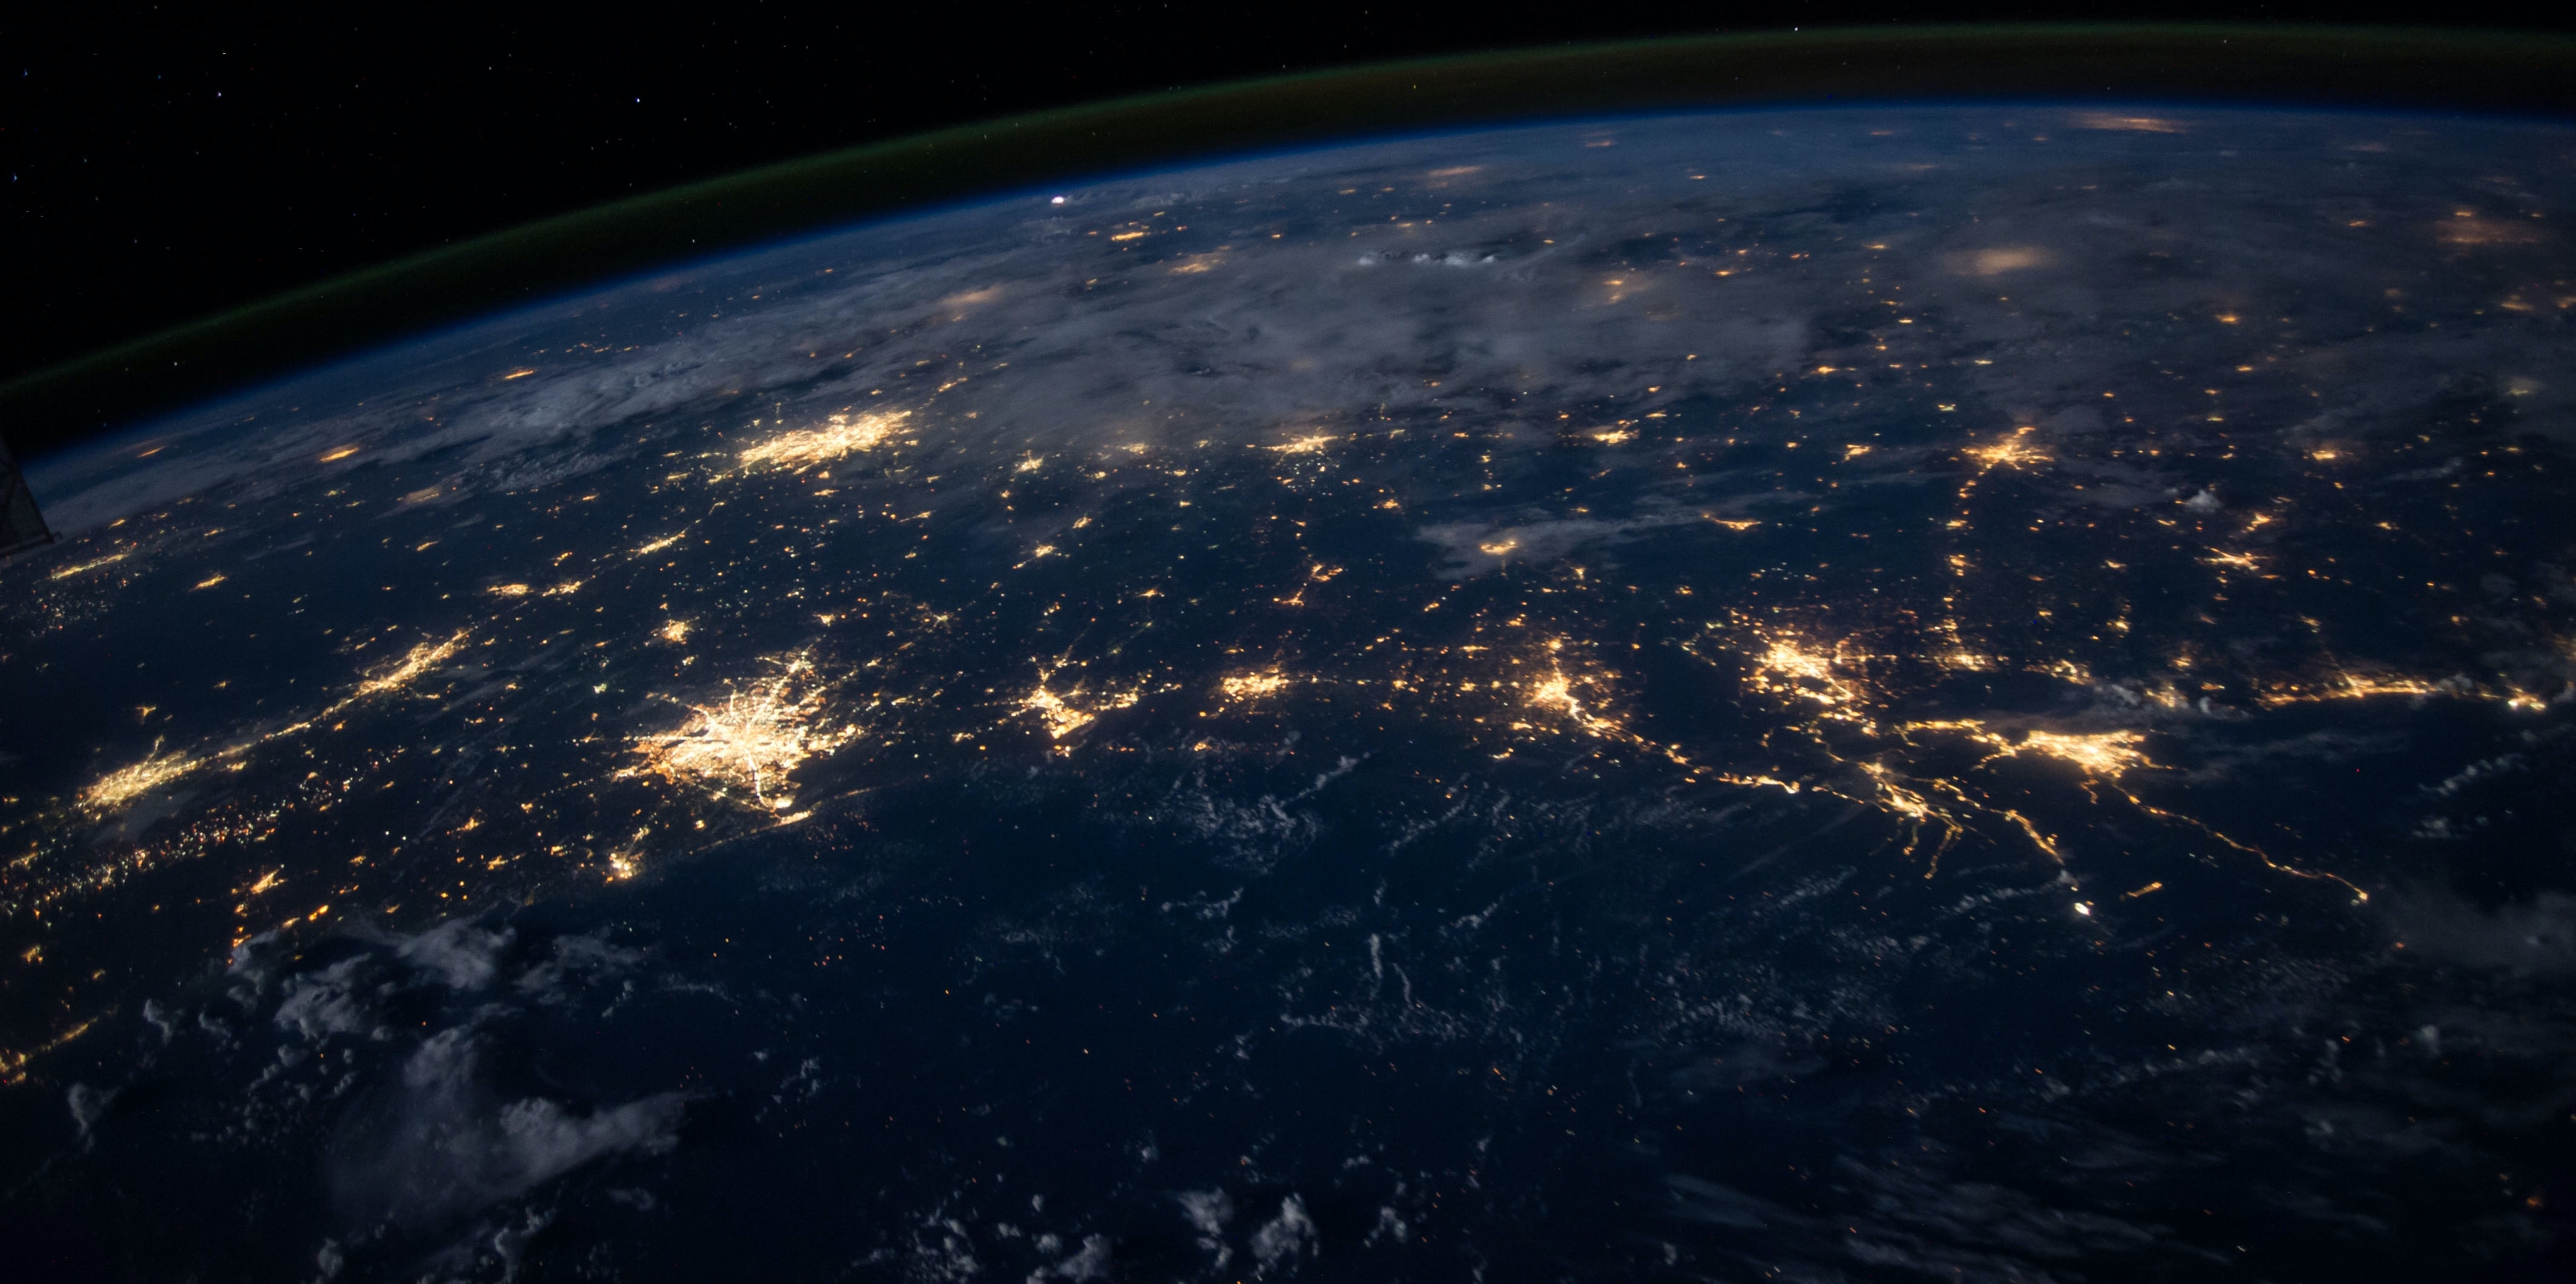
\includegraphics[width=\linewidth]{images/illustrations}
	\end{figure}
	
	\begin{flushright}
		% 标题
		{ \Huge \bfseries Physics with Coding} \hspace*{6em} \\[0.2cm]
		\rule{0.618\textwidth}{5pt} \hspace*{6em} \\[1cm]
		
		% 作者
		\LARGE\emph{\textbf{Copyright@pifuyuini}} \hspace*{4.2em}
		
	\end{flushright}
	
	% Bottom of the page
	\begin{center}
		\vfill
		
		\Large\texttt{\textcolor{fgrayblue}{Programming instruction for undergraduate physics students.}}
		
		\hspace*{\fill}
		
		{\LARGE \today}
		
		\hspace*{\fill}
	\end{center}
	
\end{titlepage} % 封面页，选用
	% !TEX root = ../main.tex

\begin{center}
	\Huge \textbf{\textcolor{fblack}{Preface}}
\end{center}

\begin{ubox}{项目计划}
	\begin{itemize}
		\item 附录：计算机基础
		\item 附录：环境的搭建与配置
		\item 附录：The missing semester 
		\item 附录：\LaTeX
		\item 附录：爬虫
		\item 附录：服务器与个人网站
		\item 附录：量子计算
		
		\item 第一部分：计算机科学导论
		\item 第二部分：数据处理与分析
		\item 第三部分：数值方法与模拟
		\item 第四部分：AI基础
		\item 第五部分：机器学习
		\item 第六部分：深度学习
		
		\item 编程语言：Python
		\item 编程语言：C++
	\end{itemize}
\end{ubox} % 前言
	
	% 目录
	\tableofcontents
	
	% 主体部分
	\mainmatter
	
	% 正文
	% !TEX root = ../main.tex

\chapter{（这是笔记名）测试笔记}
\section{（这是第一章）夜色名为温柔}

\subsection{（这是第一节）天空与你之间}

\subsubsection{（这是第一小节）萤和球棒侠}

\textbf{接下来用于测试基本文本编辑，包括各种有序列表、无序列表、行内公式以及字体颜色等：}

\begin{itemize}
	\item 开路电压是指没有外部负载连接时，热电发电装置两端的电压。根据Seebeck效应，开路电压与温差成正比，$V_{\text{oc}} = \alpha \Delta T$。
	
	\begin{itemize}
		\item \textcolor{fred}{通过实验测量，展示即使是优化过的热电装置，其效率也受到卡诺效率的限制，这直接体现了热力学第二定律。}
		\begin{itemize}
			\item \textcolor{fred}{通过实验测量，展示即使是优化过的热电装置，其效率也受到卡诺效率的限制，这直接体现了热力学第二定律。}
			\item 讨论如何通过实验设计来逼近卡诺效率，包括使用最佳材料、最佳温差和最佳负载条件。
		\end{itemize}			
		\item 讨论如何通过实验设计来逼近卡诺效率，包括使用最佳材料、最佳温差和最佳负载条件。
	\end{itemize}			
	
	\item 当热电发电装置连接到负载时，输出电压会由于内阻的存在而下降。负载电压$V_{\text{L}} = \frac{\alpha \Delta T \cdot R_{\text{L}}}{R_{\text{L}} + R_{\text{in}}}$，而输出功率是负载上消耗的功率$P_{\text{out}} = \frac{(\alpha \Delta T)^2 \cdot R_{\text{L}}}{(R_{\text{L}} + R_{\text{in}})^2}$。
	
	\item 当负载电阻等于内阻时，热电发电装置输出的功率达到最大$P_{\text{max}} = \frac{(\alpha \Delta T)^2}{4 R_{\text{in}}}$。				
\end{itemize}

\begin{enumerate}
	\item 各元件性能测量
	\begin{enumerate}
		\item \textcolor{fred}{Seebeck效应测量}：通过改变温差并测量开路电压来研究Seebeck效应，从而确定$\alpha$；
		\begin{enumerate}
			\item \textcolor{fred}{热电堆集成——电加热器与Seebeck元件，测控部分——PID控温（热端、冷端），输出电路部分（输出功率测量）。}
			\begin{enumerate}
				\item \textcolor{fred}{加热功率测控}——电流表电压表实时测控（含于PID系统中，编写相关程序）；
				\item \textcolor{fred}{输出功率测控}——电流表电压表实时测控（考虑是否编程）；
				\item 测量最大输出功率——改变输出电路的负载；
				\item 测量最大输出效率——改变温差与负载，优化其它部分；
				\item 探究如何测量热端的损失。
			\end{enumerate}
		\end{enumerate}
		\item 器件内阻的测量与影响：内阻对热电转换效率有重要影响，了解并优化内阻对提高热机性能是必要的；
		\item 考虑测量电加热器的加热功率（以及其它元件性能，如Peltier效应）。
	\end{enumerate}
	
	\item \textcolor{fred}{搭建热机}
	
	\item 负载与效率测量
	
	
	\item 热力学第二定律的展示
	\begin{itemize}
		\item \textcolor{fred}{通过实验测量，展示即使是优化过的热电装置，其效率也受到卡诺效率的限制，这直接体现了热力学第二定律。}
		\item 讨论如何通过实验设计来逼近卡诺效率，包括使用最佳材料、最佳温差和最佳负载条件。
	\end{itemize}			
	
	\item 结论与进一步的探索
	\begin{itemize}
		\item 比较热机效率与理论卡诺效率的差异，讨论可能的优化途径和技术挑战；
		\item 探究各部分如何\textcolor{fred}{优化}（热电堆——减小散热，增大温差，冷热端优化；测控——优化控温算法，改进实时测量程序；输出电路部分——减小散热，考虑Thomson效应的影响；理论建模——估算散热进一步修正）。
	\end{itemize}
\end{enumerate}

\textbf{接下来用于测试图片、表格以及带编号公式，并且考虑它们的引用：}

\textbf{这是带编号公式：}

\begin{equation}
	V_{\text{oc}} = \alpha \Delta T
	\label{eq:test}
\end{equation}

来看看\cref{eq:test}。

\textbf{这是表格：}

\begin{table}[h]
	\centering
	\caption{高级控温算法的比较}
	\label{tab:tab1}
	\begin{tabular}{|c|c|c|}
		\hline
		控温算法 & 优点 & 缺点 \\
		\hline
		PID 控制 & 简单、易实现 & 性能有限，难以处理复杂系统 \\
		\hline
		模糊控制 & 不需要精确模型，适应性强 & 规则设计复杂，性能依赖于规则质量 \\
		\hline
		模型预测控制 & 最优性能，多变量处理 & 计算量大，依赖系统模型 \\
		\hline
		自适应控制 & 参数自调整，适应性强 & 实现复杂，收敛性问题 \\
		\hline
		神经网络控制 & 非线性处理能力强 & 训练复杂，数据需求大 \\
		\hline
		最优控制 & 理论性能优 & 实现复杂，计算量大 \\
		\hline
	\end{tabular}			
\end{table}

来看看\cref{tab:tab1}。

\clearpage
\textbf{这是图片：}

\begin{figure}[htbp]
	\centering
	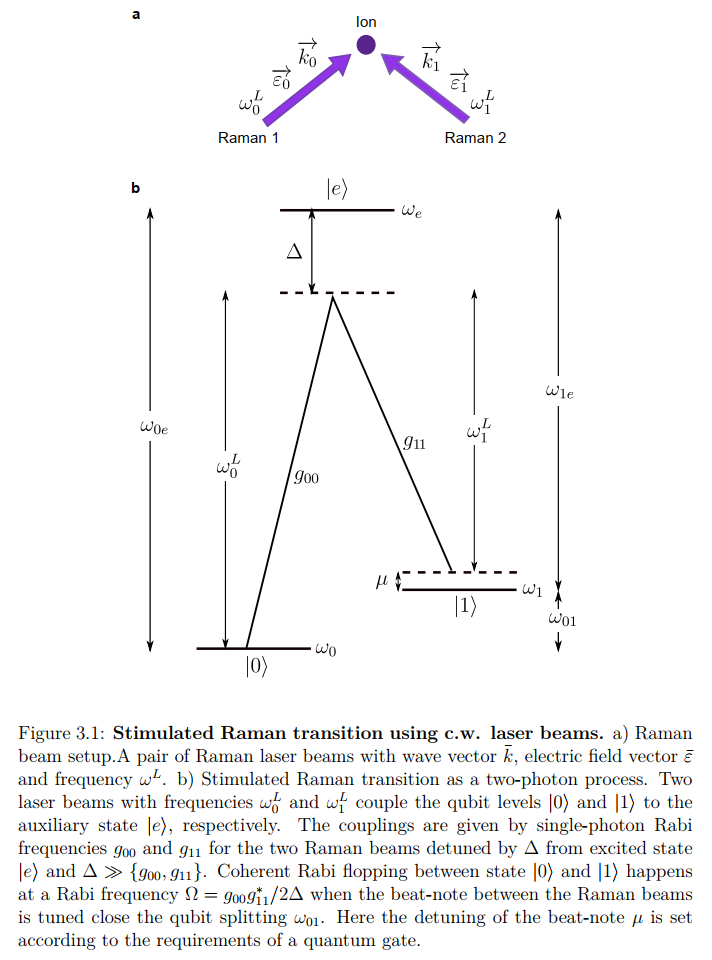
\includegraphics[width=0.7\textwidth]{Stimulated Raman transition using c.w. laser beams.png}
	\caption{Stimulated Raman transition using c.w. laser beams}
	\label{fig:Stimulated Raman transition using c.w. laser beams}
\end{figure}

来看看\cref{fig:Stimulated Raman transition using c.w. laser beams}。

\clearpage
\subsubsection{（这是第二小节）星和猎手}

\textbf{这个公式用于展示带编号公式的编号规则：}

\begin{equation}
	V_{\text{oc}} = \alpha \Delta T
\end{equation}

\textbf{接下来将用于展示各种各样的自定义环境：}

\textbf{首先是几种颜色盒子：}

\textbf{这是要点：}

\begin{keypoint}[label=key:firefly]
	这是一段关于流萤的文本。
\end{keypoint}

引用示例：\cref{key:firefly}。

\textbf{这是通用框架，通常不引用：}

\begin{ubox}{约会的小曲}
	若我不曾见过太阳、
	使一颗心免于哀伤。
\end{ubox}

\textbf{这是高亮：}

\highlight{流萤！}

\textbf{这是代码环境：}

\begin{macbox}{</>Python}
	\begin{lstlisting}[style=pythonstyle]
		# 示例代码
		import matplotlib.pyplot as plt
		import numpy as np
		
		# Data for plotting
		t = np.arange(0.0, 2.0, 0.01)
		s = 1 + np.sin(2 * np.pi * t)
		
		fig, ax = plt.subplots()
		ax.plot(t, s)
		
		ax.set(xlabel='time (s)', ylabel='voltage (mV)',
		title='About as simple as it gets, folks')
		ax.grid()
		
		fig.savefig("test.png")
		plt.show()
	\end{lstlisting}
\end{macbox}
 % 展示模版的效果，方便一些指令的查询
	%% !TEX root = ../main.tex

\chapter{Data Processing \& Analysis}

思考：有了AI辅助后，从能做什么转向到\highlight{要做些什么}。

所谓“思路构建”。 % 数据分析
	% !TEX root = ../main.tex

\chapter{Fast Fourier Transform (FFT)}

\section{The Principle and Implementation of Discrete Fourier Transform}

\section{The Principles of FFT}

\section{Optimization of FFT}

\section{High-performance FFT} % （临时）FFT实现
	%% !TEX root = ../main.tex

\chapter{AI Fundamentals} % AI基础
	%% !TEX root = ../main.tex

\chapter{Machine Learning}



\section{Introduction}
What is machine learning?



\section{Linear Model}
\section{Decision Tree}
\section{Neural Networks}
\section{Support Vector Machine}
\section{Bayesian Classifier}
\section{Ensemble Learning}
\section{Clustering}
\section{Dimensionality Reduction \& Metric Learning}
\section{Feature Selection \& Sparse Learning}
\section{Semi-supervised Learning}
\section{Probabilistic Graphical Models}
\section{Reinforcement Learning} % 机器学习
	
	% 参考文献
	% !TEX root = main.tex

\begin{thebibliography}{99}
	%\bibitem{a}作者. \emph{文献}[M]. 地点:出版社,年份.\cite{ref1}
	\bibitem{a}作者. \emph{文献}[M]. 地点:出版社,年份.
\end{thebibliography}
	
	% 附录

	
\end{document}